\documentclass[aspectratio=169]{beamer}

% Theme and Color Scheme
\usetheme{Madrid}
\usecolortheme{beaver}

% Packages
\usepackage[utf8]{inputenc}
\usepackage{graphicx}
\usepackage{tikz}
% \usepackage{fontawesome}
\usepackage{xcolor}
\usepackage{amsmath}
\usepackage{array}

% Title Information
\title[CSC111: Unit 2]{CSC111: Electronics Computer}
\subtitle{Turing Model, Von Neumann Model \& Data Processing}
\author{Computer Science Department}
\institute{University}
\date{\today}

% Custom Colors
\definecolor{darkblue}{RGB}{0,51,102}
\definecolor{lightblue}{RGB}{173,216,230}
\definecolor{turingcolor}{RGB}{34,139,34}
\definecolor{voncolor}{RGB}{220,20,60}


% Theme and Color Scheme
\usetheme{Madrid}
\usecolortheme{beaver}

% Packages
\usepackage[utf8]{inputenc}
\usepackage{graphicx}
\usepackage{tikz}
\usepackage{fontawesome5}
\usepackage{xcolor}



\definecolor{myNewColorA}{RGB}{206,008,20} %#put red here
\definecolor{myNewColorB}{RGB}{26,168,217} %Blue106,172,150
\definecolor{myNewColorC}{RGB}{245, 233, 85} %26,163,217
\setbeamercolor*{palette primary}{bg=myNewColorC}
\setbeamercolor*{palette secondary}{bg=myNewColorB, fg=white}
\setbeamercolor*{palette tertiary}{bg=myNewColorA, fg=white}
\setbeamercolor*{titlelike}{fg=myNewColorA}
\setbeamercolor*{title}{bg=myNewColorA, fg=white}
\setbeamercolor*{item}{fg=myNewColorA}
\setbeamercolor*{caption name}{fg=myNewColorA}
\usefonttheme{professionalfonts}
\usepackage{natbib}
\usepackage{hyperref}

% Title Information
\titlegraphic{
\includegraphics[height=1.5cm]{UNESWA_logo.png}}

\setbeamerfont{title}{size=\large}
\setbeamerfont{subtitle}{size=\small}
\setbeamerfont{author}{size=\small}
\setbeamerfont{date}{size=\small}
\setbeamerfont{institute}{size=\small}
\title[University of Eswatini]{Introduction to Computer Science
}
\subtitle{CSC111}
\author[J.S.D]{Mr. Johnson Dlamini}

\institute[jsdlamini@uniswa.sz]{ The University of Eswatini}
\date

% Custom Colors
\definecolor{darkblue}{RGB}{0,51,102}
\definecolor{lightblue}{RGB}{173,216,230}

\AtBeginSection[]{
  \begin{frame}
  \vfill
  \centering
  \begin{beamercolorbox}[sep=8pt,center,shadow=true,rounded=true]{title}
    \usebeamerfont{title}\insertsectionhead\par%
  \end{beamercolorbox}
  \vfill
  \end{frame}
}

\begin{document}

% Title Slide
\frame{\titlepage}

% Table of Contents
\begin{frame}{Outline}
    \tableofcontents
\end{frame}

% Section 1: Introduction
\section{Introduction}

\begin{frame}{Unit Overview}
    \begin{columns}
        \begin{column}{0.6\textwidth}
            \textbf{What we'll explore:}
            \begin{itemize}
                \item Turing Model vs Von Neumann Model
                \item Computer classification by purpose
                \item Data, Information, and Processing
                \item Types of data processing
                \item Methods of data processing
            \end{itemize}
        \end{column}
        \begin{column}{0.4\textwidth}
            \centering
            % Placeholder for computer models image
            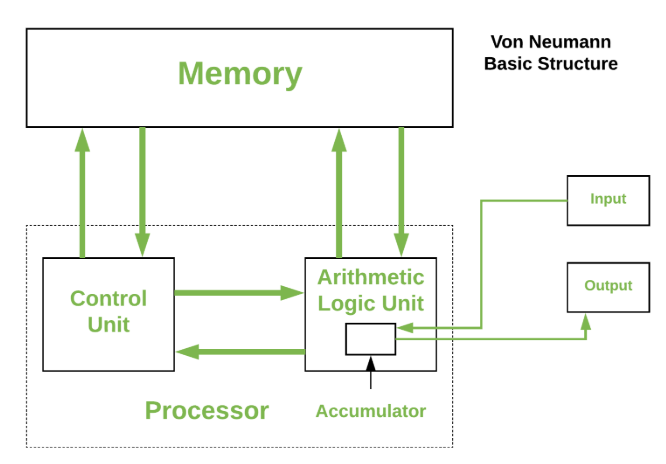
\includegraphics[width=\textwidth]{images/ch2/computer_models.png}
            \small{\textit{Computer Architecture Models}}
        \end{column}
    \end{columns}
    
    \vspace{0.5cm}
    \begin{alertblock}{Learning Focus}
        Understanding the theoretical foundations of computer architecture and data processing methodologies.
    \end{alertblock}
\end{frame}

\begin{frame}{Learning Outcomes}
    \textbf{After studying this unit, you should be able to:}
    \begin{enumerate}
        \item \faCheckCircle\, Describe the different models of a computer
        \item \faCheckCircle\, Give definitions of Data, Information and data processing
        \item \faCheckCircle\, State the different types of data processing
        \item \faCheckCircle\, Explain the methods of data processing
    \end{enumerate}
    
    \vspace{0.5cm}
    \begin{exampleblock}{Key Concepts}
        We'll examine how computers process information from theoretical and practical perspectives.
    \end{exampleblock}
\end{frame}

% Section 2: Turing Model
\section{Turing Model}

\begin{frame}{Alan Turing and the Universal Machine}
    \begin{columns}
        \begin{column}{0.5\textwidth}
            \textbf{Historical Context:}
            \begin{itemize}
                \item \textbf{Year:} 1936
                \item \textbf{Creator:} Alan Turing
                \item \textbf{Concept:} First universal computational device
                \item \textbf{Vision:} All computation performed by machine
            \end{itemize}
            
            \vspace{0.3cm}
            \begin{block}{Turing's Projection}
                "All computation should be performed by a machine called \textcolor{turingcolor}{\textbf{Turing Machine}}"
            \end{block}
        \end{column}
        \begin{column}{0.5\textwidth}
            % Placeholder for Alan Turing image
            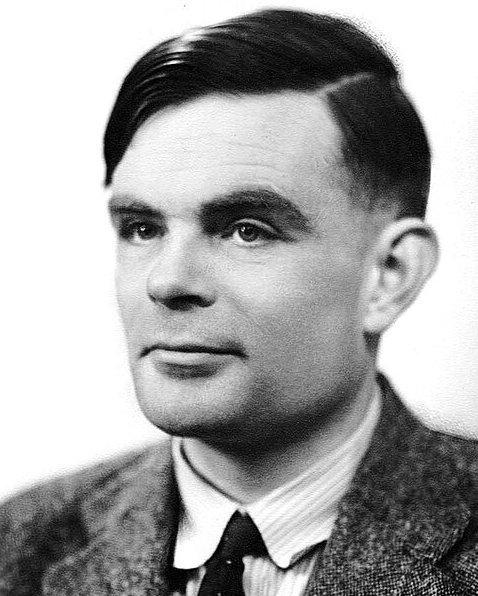
\includegraphics[width=0.7\textwidth]{images/ch2/alan_turing.png} \\
            \small{\textit{Alan Turing (1912-1954)\\Mathematician \& Computer Scientist}}
        \end{column}
    \end{columns}
\end{frame}

\begin{frame}{Turing Machine Components}
    \begin{definition}
        A Turing machine is a theoretical model of computation that includes a tape extending infinitely in both directions.
    \end{definition}
    
    \vspace{0.5cm}
    \textbf{Key Components:}
    \begin{enumerate}
        \item \textbf{Infinite Tape:} Divided into cells, each containing one symbol
        \item \textbf{Tape Alphabet:} Finite set of symbols including:
        \begin{itemize}
            \item Special symbol \texttt{b} (for blank)
            \item Usually symbols \texttt{0} and \texttt{1}
            \item Limited number of other symbols
        \end{itemize}
        \item \textbf{Read/Write Head:} Reads one cell at a time and writes symbols
        \item \textbf{States:} Finite number k of states (1, 2, 3, 4, ..., k)
    \end{enumerate}
\end{frame}

\begin{frame}{Turing Machine Tape Structure}
    \begin{center}
        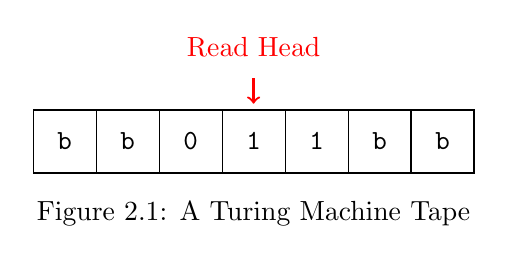
\begin{tikzpicture}[scale=0.8]
            % Draw tape cells
            \foreach \x in {0,1,2,3,4,5,6}
            {
                \draw (\x,0) rectangle (\x+1,1);
            }
            
            % Add symbols
            \node at (0.5,0.5) {\texttt{b}};
            \node at (1.5,0.5) {\texttt{b}};
            \node at (2.5,0.5) {\texttt{0}};
            \node at (3.5,0.5) {\texttt{1}};
            \node at (4.5,0.5) {\texttt{1}};
            \node at (5.5,0.5) {\texttt{b}};
            \node at (6.5,0.5) {\texttt{b}};
            
            % Add arrow pointing to current cell
            \draw[->, thick, red] (3.5,1.5) -- (3.5,1.1);
            \node[above, red] at (3.5,1.7) {Read Head};
            
            % Add labels
            \node[below] at (3.5,-0.3) {Figure 2.1: A Turing Machine Tape};
        \end{tikzpicture}
    \end{center}
    
    \vspace{0.5cm}
    \begin{block}{Tape Functions}
        \begin{itemize}
            \item \textbf{Input:} Holds input as finite string of nonblank symbols
            \item \textbf{Output:} Machine writes output using same alphabet
            \item \textbf{Memory:} Serves as storage for computation
        \end{itemize}
    \end{block}
\end{frame}

\begin{frame}{Turing Machine Operations}
    \textbf{Single Primitive Operation - Three Actions:}
    
    \begin{enumerate}
        \item \textbf{Write:} Write a symbol in the cell (replacing existing symbol)
        \item \textbf{State Change:} Go into a new state (might be same as current)
        \item \textbf{Move:} Move read head one cell left or right
    \end{enumerate}
    
    \vspace{0.5cm}
    \begin{block}{Instruction Format}
        \texttt{If (you are in state i) and (you are reading symbol j) then}
        \begin{itemize}
            \item Write symbol k onto the tape
            \item Go into state s
            \item Move in direction d (left or right)
        \end{itemize}
    \end{block}
    
    \vspace{0.3cm}
    \begin{exampleblock}{State Analogy}
        A state can be thought of as a condition - like your "hungry state" based on recent meals.
    \end{exampleblock}
\end{frame}

\begin{frame}{Turing Machine Instruction Example}
    \textbf{Sample Instruction:}
    \begin{block}{Instruction}
        If (you are in state 1) and (you are reading symbol 0) then
        \begin{itemize}
            \item Write symbol 1 onto the tape
            \item Go into state 2  
            \item Move right
        \end{itemize}
    \end{block}
    
    % \vspace{0.1cm}
    \textbf{Before Execution:}
    \begin{center}
        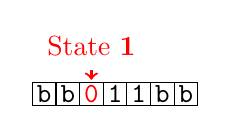
\begin{tikzpicture}[scale=0.3]
            \foreach \x in {0,1,2,3,4,5,6}
            {
                \draw (\x,0) rectangle (\x+1,1);
            }
            \node at (0.5,0.5) {\texttt{b}};
            \node at (1.5,0.5) {\texttt{b}};
            \node at (2.5,0.5) {\textcolor{red}{\textbf{\texttt{0}}}};
            \node at (3.5,0.5) {\texttt{1}};
            \node at (4.5,0.5) {\texttt{1}};
            \node at (5.5,0.5) {\texttt{b}};
            \node at (6.5,0.5) {\texttt{b}};
            \draw[->, thick, red] (2.5,1.5) -- (2.5,1.1);
            \node[above, red] at (2.5,1.7) {State \textbf{1}};
        \end{tikzpicture}
    \end{center}
    
    \textbf{After Execution:}
    \begin{center}
        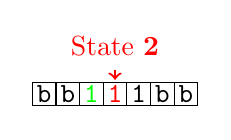
\begin{tikzpicture}[scale=0.3]
            \foreach \x in {0,1,2,3,4,5,6}
            {
                \draw (\x,0) rectangle (\x+1,1);
            }
            \node at (0.5,0.5) {\texttt{b}};
            \node at (1.5,0.5) {\texttt{b}};
            \node at (2.5,0.5) {\textcolor{green}{\textbf{\texttt{1}}}};
            \node at (3.5,0.5) {\textcolor{red}{\textbf{\texttt{1}}}};
            \node at (4.5,0.5) {\texttt{1}};
            \node at (5.5,0.5) {\texttt{b}};
            \node at (6.5,0.5) {\texttt{b}};
            \draw[->, thick, red] (3.5,1.5) -- (3.5,1.1);
            \node[above, red] at (3.5,1.7) {State \textbf{2}};
        \end{tikzpicture}
    \end{center}
\end{frame}

\begin{frame}{Five Components of Turing Machine}
    \begin{columns}
        \begin{column}{0.45\textwidth}
            \textbf{Turing Machine 5-Tuple:}
            \begin{enumerate}
                \item \textcolor{turingcolor}{\textbf{Current state}}
                \item \textcolor{turingcolor}{\textbf{Current symbol}}
                \item \textcolor{turingcolor}{\textbf{Next symbol}}
                \item \textcolor{turingcolor}{\textbf{Next state}}
                \item \textcolor{turingcolor}{\textbf{Direction of move}}
            \end{enumerate}
            
            \vspace{0.5cm}
            \begin{exampleblock}{5-Tuple Notation}
                \texttt{(1,0,1,2,R)} means:
                \small{In state 1, reading 0, write 1, go to state 2, move right}
            \end{exampleblock}
        \end{column}
        \begin{column}{0.5\textwidth}
            \textbf{Another Example:}
            \begin{block}{Instruction (2,1,1,2,L)}
                If (state 2) and (reading symbol 1) then
                \begin{itemize}
                    \item Write symbol 1
                    \item Go into state 2  
                    \item Move left
                \end{itemize}
            \end{block}
            
            \vspace{0.3cm}
            \begin{alertblock}{Note}
                This writes the same symbol and stays in same state, but moves left.
            \end{alertblock}
        \end{column}
    \end{columns}
\end{frame}

% Section 3: Data Processing Concepts
\section{Data Processing}

\begin{frame}{Understanding Data Processing}
    \begin{definition}
        \textbf{Data Processing} is the process of converting data into information.
    \end{definition}
    
    \vspace{0.5cm}
    \begin{columns}
        \begin{column}{0.45\textwidth}
            \begin{block}{Data}
                Collection of raw facts and figures
                \begin{itemize}
                    \item Student admission forms
                    \item Examination scores
                    \item Census data
                \end{itemize}
            \end{block}
        \end{column}
        \begin{column}{0.5\textwidth}
            \begin{block}{Information}
                Processed data organized meaningfully
                \begin{itemize}
                    \item Student results
                    \item Census reports
                    \item Scholarship lists
                \end{itemize}
            \end{block}
        \end{column}
    \end{columns}
    
    \vspace{0.5cm}
    \begin{center}
        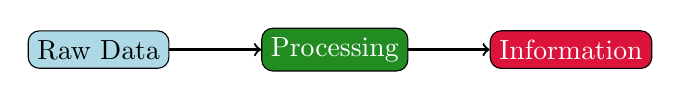
\begin{tikzpicture}
            \node[draw, rounded corners, fill=lightblue] (data) at (0,0) {Raw Data};
            \node[draw, rounded corners, fill=turingcolor, text=white] (process) at (3,0) {Processing};
            \node[draw, rounded corners, fill=voncolor, text=white] (info) at (6,0) {Information};
            \draw[->, thick] (data) -- (process);
            \draw[->, thick] (process) -- (info);
        \end{tikzpicture}
    \end{center}
\end{frame}

\begin{frame}{Types of Data Processing}
    \textbf{Three Main Types:}
    
    \begin{enumerate}
        \item \textbf{\faHandPaper\, Manual Data Processing}
        \item \textbf{\faCog\, Mechanical Data Processing}
        \item \textbf{\faLaptop\, Electronic Data Processing}
    \end{enumerate}
    
    \vspace{0.5cm}
    \begin{center}
        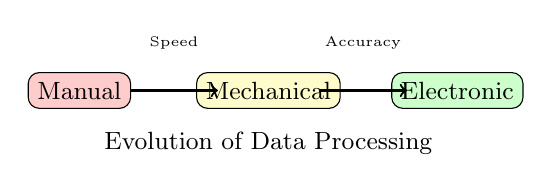
\begin{tikzpicture}[scale=0.8]
            % Evolution timeline
            \node[draw, rounded corners, fill=red!20] at (0,0) {\small{Manual}};
            \node[draw, rounded corners, fill=yellow!20] at (3,0) {\small{Mechanical}};
            \node[draw, rounded corners, fill=green!20] at (6,0) {\small{Electronic}};
            
            \draw[->, thick] (0.8,0) -- (2.2,0);
            \draw[->, thick] (3.8,0) -- (5.2,0);
            
            \node[above] at (1.5,0.5) {\tiny{Speed}};
            \node[above] at (4.5,0.5) {\tiny{Accuracy}};
            \node[below] at (3,-0.5) {\small{Evolution of Data Processing}};
        \end{tikzpicture}
    \end{center}
\end{frame}

\begin{frame}{Manual Data Processing}
    \begin{definition}
        Processing data using hand, paper, brain and other supporting materials without machines.
    \end{definition}
    
    \vspace{0.5cm}
    \begin{columns}
        \begin{column}{0.5\textwidth}
            \textbf{Characteristics:}
            \begin{itemize}
                \item No electronic devices
                \item Manual calculations
                \item Human-powered operations
                \item Paper-based records
            \end{itemize}
            
            \vspace{0.3cm}
            \textbf{\textcolor{green}{Advantages:}}
            \begin{itemize}
                \item[\faCheck] Cost effective
            \end{itemize}
        \end{column}
        \begin{column}{0.5\textwidth}
            \textbf{\textcolor{red}{Disadvantages:}}
            \begin{itemize}
                \item[\faTimes] Slowest method
                \item[\faTimes] Prone to errors
                \item[\faTimes] Not programmable
                \item[\faTimes] Limited scalability
            \end{itemize}
            
            % \vspace{0.3cm}
            % Placeholder for manual processing image
            % \includegraphics[width=0.5\textwidth]{manual_processing.png}
        \end{column}
    \end{columns}
\end{frame}

\begin{frame}{Mechanical Data Processing}
    \begin{definition}
        Data processing using mechanical devices or simple electronic devices like calculators and typewriters.
    \end{definition}
    
    \vspace{0.5cm}
    \begin{columns}
        \begin{column}{0.5\textwidth}
            \textbf{\textcolor{green}{Advantages:}}
            \begin{itemize}
                \item[\faCheck] More accurate than manual
                \item[\faCheck] Faster than manual
                \item[\faCheck] Fewer errors than manual
            \end{itemize}
        \end{column}
        \begin{column}{0.5\textwidth}
            \textbf{\textcolor{red}{Disadvantages:}}
            \begin{itemize}
                \item[\faTimes] More expensive than manual
                \item[\faTimes] Not programmable
                \item[\faTimes] No storage space
            \end{itemize}
        \end{column}
    \end{columns}
    
    \vspace{0.5cm}
    \begin{exampleblock}{Use Cases}
        Suitable when processing needs are simple and mechanical devices can handle the workload effectively.
    \end{exampleblock}
    
    % \begin{center}
    %     % Placeholder for mechanical devices image
    %     \includegraphics[width=0.4\textwidth]{mechanical_devices.png}
    % \end{center}
\end{frame}

\begin{frame}[fragile]{Electronic Data Processing}
 \smaller
    \begin{definition}
        Modern technique using computers - the fastest and most reliable method with highest accuracy.
    \end{definition}
    
    % \vspace{0.3cm}
    \begin{columns}
        \begin{column}{0.5\textwidth}
            \textbf{\textcolor{green}{Advantages:}}
            \begin{itemize}
                \item[\faCheck] Fastest processing
                \item[\faCheck] Most efficient
                \item[\faCheck] Large volume handling
                \item[\faCheck] Accurate results (GIGO)
                \item[\faCheck] Large storage capacity
            \end{itemize}
        \end{column}
        \begin{column}{0.5\textwidth}
            \textbf{\textcolor{red}{Disadvantages:}}
            \begin{itemize}
                \item[\faTimes] Most expensive
                \item[\faTimes] Requires training
                \item[\faTimes] Technical complexity
                \item[\faTimes] Maintenance needs
            \end{itemize}
        \end{column}
    \end{columns}
    
    % \vspace{0.3cm}

    \begin{columns}
        \begin{column}{0.45\textwidth}
           % \smaller
    \begin{block}{GIGO Principle}
       \tiny{ \textbf{Garbage In, Garbage Out} - Computers produce accurate results only when input data and instructions are correct.}
    \end{block}
    
        \end{column}
        \begin{column}{0.5\textwidth}
  \begin{exampleblock}{Modern Usage}
       \tiny{  Employed in most agencies and organizations for data processing tasks.}
    \end{exampleblock}
        \end{column}
\end{columns}
        
   
    
  
\end{frame}

\begin{frame}{Methods of Data Processing}
    \textbf{Five Primary Methods:}
    
    \begin{enumerate}
        \item \faStream\, \textbf{Batch Processing}
        \begin{itemize}
            \item Process data in groups/batches
            \item Suitable for large volumes
            \item Non-interactive processing
        \end{itemize}
        
        \item \faClock\, \textbf{Real-time Processing}
        \begin{itemize}
            \item Immediate processing
            \item Instant results required
            \item Interactive systems
        \end{itemize}
        
        \item \faGlobe\, \textbf{Online Processing}
        \begin{itemize}
            \item Network-based processing
            \item Remote data access
            \item Web-enabled systems
        \end{itemize}
    \end{enumerate}
\end{frame}

\begin{frame}{Methods of Data Processing (Continued)}
    \begin{enumerate}
        \setcounter{enumi}{3}
        \item \faMicrochip\, \textbf{Multiprocessing}
        \begin{itemize}
            \item Multiple processors working simultaneously
            \item Parallel processing capabilities
            \item Enhanced performance
        \end{itemize}
        
        \item \faShareAlt\, \textbf{Time-sharing}
        \begin{itemize}
            \item Multiple users share computing resources
            \item Scheduled processor allocation
            \item Efficient resource utilization
        \end{itemize}
    \end{enumerate}
    
    \vspace{0.5cm}
    \begin{center}
        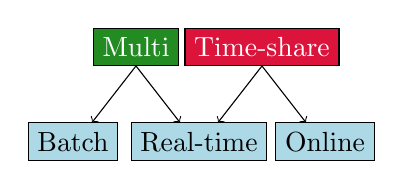
\begin{tikzpicture}[scale=0.8]
            \node[draw, fill=lightblue] at (0,0) {Batch};
            \node[draw, fill=lightblue] at (2,0) {Real-time};
            \node[draw, fill=lightblue] at (4,0) {Online};
            \node[draw, fill=turingcolor, text=white] at (1,1.5) {Multi};
            \node[draw, fill=voncolor, text=white] at (3,1.5) {Time-share};
            
            \draw[->] (1,1.2) -- (0.3,0.3);
            \draw[->] (1,1.2) -- (1.7,0.3);
            \draw[->] (3,1.2) -- (2.3,0.3);
            \draw[->] (3,1.2) -- (3.7,0.3);
        \end{tikzpicture}
    \end{center}
\end{frame}

% Section 4: Computer Classification
\section{Computer Classification}

\begin{frame}{Computer Classification by Purpose}
    \textbf{Two Main Categories:}
    
    \begin{columns}
        \begin{column}{0.45\textwidth}
            \begin{block}{General-Purpose Computer}
                \textbf{Characteristics:}
                \begin{itemize}
                    \item Perform different tasks
                    \item Programmable for various applications
                    \item Flexible and adaptable
                \end{itemize}
                
                \textbf{Examples:}
                \begin{itemize}
                    \item Business centers
                    \item Universities
                    \item Research institutes
                \end{itemize}
            \end{block}
        \end{column}
        \begin{column}{0.5\textwidth}
            \begin{block}{Special-Purpose Computer}
                \textbf{Characteristics:}
                \begin{itemize}
                    \item Perform single specific task
                    \item Lacks general programming capability
                    \item Optimized for specific function
                \end{itemize}
                
                \textbf{Examples:}
                \begin{itemize}
                    \item Bank transaction systems
                    \item Weather forecasting
                    \item Manufacturing control
                    \item Library automation
                \end{itemize}
            \end{block}
        \end{column}
    \end{columns}
\end{frame}

\begin{frame}{Turing Model and Computer Purpose}
    \begin{block}{Turing Model Support}
        The Turing model supports general-purpose computers with electronic data processing capabilities for the 4th Industrial Revolution.
    \end{block}
    
    % \vspace{0.5cm}
    \textbf{Three Turing Model Scenarios:}
    \begin{enumerate}
        \item \textbf{Same program + Different input data} = Different output
        \item \textbf{Same input data + Different program} = Different output  
        \item \textbf{Same input data + Same program} = Same output
    \end{enumerate}
    
    % \vspace{0.5cm}
    \begin{center}
        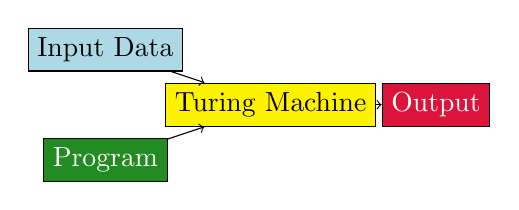
\begin{tikzpicture}[scale=0.7]
            % Input
            \node[draw, fill=lightblue] (input) at (0,1) {Input Data};
            \node[draw, fill=turingcolor, text=white] (program) at (0,-1) {Program};
            
            % Process
            \node[draw, fill=yellow] (turing) at (3,0) {Turing Machine};
            
            % Output
            \node[draw, fill=voncolor, text=white] (output) at (6,0) {Output};
            
            % Arrows
            \draw[->] (input) -- (turing);
            \draw[->] (program) -- (turing);
            \draw[->] (turing) -- (output);
        \end{tikzpicture}
    \end{center}
    
    \begin{definition}
        \textbf{Turing Machine:} A machine with the capacity of computing anything that is computable.
    \end{definition}
\end{frame}

% Section 5: Von Neumann Model
\section{Von Neumann Model}

\begin{frame}{Von Neumann Architecture}
    \begin{columns}
        \begin{column}{0.5\textwidth}
            \textbf{Historical Background:}
            \begin{itemize}
                \item \textbf{Period:} 1944-1945
                \item \textbf{Inventor:} John Von Neumann
                \item \textbf{Key Insight:} Programs and data are logically the same
                \item \textbf{Proposal:} Store programs in memory
            \end{itemize}
        \end{column}
        \begin{column}{0.5\textwidth}
            % Placeholder for Von Neumann image
            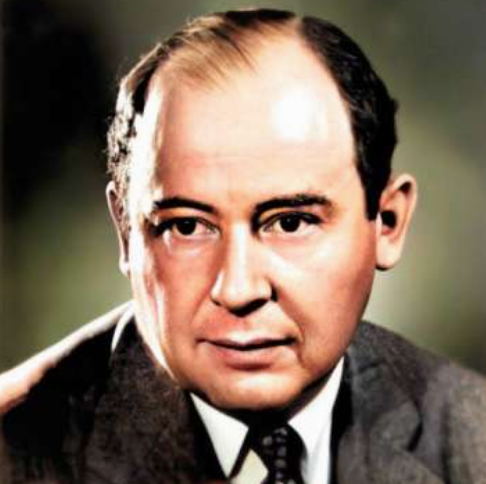
\includegraphics[width=\textwidth]{images/ch2/von_neumann.png}
            \small{\textit{John Von Neumann\\(1903-1957)}}
        \end{column}
    \end{columns}
    
    \vspace{0.5cm}
    \begin{block}{Von Neumann Principle}
        Since programs and data are logically the same, \textbf{programs should be stored in computer memory} alongside data.
    \end{block}
    
    \begin{exampleblock}{Modern Impact}
        This principle forms the foundation of modern computer architecture.
    \end{exampleblock}
\end{frame}

\begin{frame}{Von Neumann Four Subsystems}
    \textbf{Computer Hardware Divisions:}
    
    \begin{enumerate}
        \item \faMemory\, \textbf{Memory Unit}
        \begin{itemize}
            \item Stores both programs and data
            \item Primary storage system
        \end{itemize}
        
        \item \faCalculator\, \textbf{Arithmetic Logic Unit (ALU)}
        \begin{itemize}
            \item Performs mathematical operations
            \item Executes logical operations
        \end{itemize}
        
        \item \faCogs\, \textbf{Control Unit (CU)}
        \begin{itemize}
            \item Controls and coordinates operations
            \item Manages instruction execution
        \end{itemize}
        
        \item \faExchangeAlt\, \textbf{Input/Output System}
        \begin{itemize}
            \item Interfaces with external devices
            \item Handles data transfer
        \end{itemize}
    \end{enumerate}
\end{frame}

\begin{frame}{Von Neumann Architecture Diagram}
    \begin{center}
        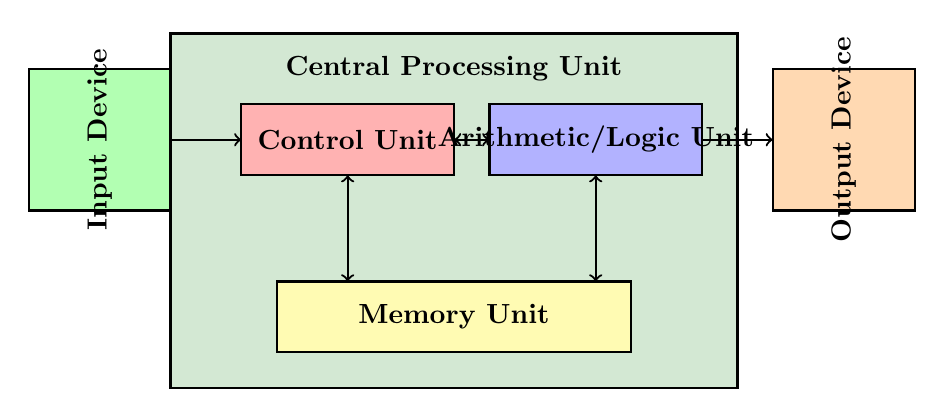
\begin{tikzpicture}[scale=0.9]
            % Main frame
            \draw[thick, fill=turingcolor!20] (-1,-3) rectangle (7,2);
            \node at (3,1.5) {\textbf{Central Processing Unit}};
            
            % Control Unit
            \draw[thick, fill=red!30] (0,0) rectangle (3,1);
            \node at (1.5,0.5) {\textbf{Control Unit}};
            
            % ALU
            \draw[thick, fill=blue!30] (3.5,0) rectangle (6.5,1);
            \node at (5,0.5) {\textbf{Arithmetic/Logic Unit}};
            
            % Memory Unit
            \draw[thick, fill=yellow!30] (0.5,-2.5) rectangle (5.5,-1.5);
            \node at (3,-2) {\textbf{Memory Unit}};
            
            % Input Device
            \draw[thick, fill=green!30] (-3,-0.5) rectangle (-1,1.5);
            \node[rotate=90] at (-2,0.5) {\textbf{Input Device}};
            
            % Output Device
            \draw[thick, fill=orange!30] (7.5,-0.5) rectangle (9.5,1.5);
            \node[rotate=90] at (8.5,0.5) {\textbf{Output Device}};
            
            % Arrows
            \draw[->, thick] (-1,0.5) -- (0,0.5);
            \draw[->, thick] (6.5,0.5) -- (7.5,0.5);
            \draw[<->, thick] (1.5,-1.5) -- (1.5,0);
            \draw[<->, thick] (5,-1.5) -- (5,0);
            \draw[<->, thick] (3,0.5) -- (3.5,0.5);
        \end{tikzpicture}
    \end{center}
    
    \vspace{0.3cm}
    \begin{alertblock}{Stored Program Concept}
        Both data and instructions are stored in the same memory system, allowing for programmable and flexible computation.
    \end{alertblock}
\end{frame}

% Section 6: Activities and Summary
\section{Activities and Summary}

\begin{frame}{Learning Activities}
    \textbf{Practice Questions:}
    \begin{enumerate}
        \item Is Pascaline Calculator computer based on Turing Model?
        \item What role is Turing model expected to play when a computer is defined as a data processor?
        \item Consider a Turing machine with five instructions - determine output for given tape
        \item What qualifies a computer to be referred to as a Data Processor?
        \item Can small and large computers perform the same tasks? Discuss
        \item Differentiate between Turing and Von Neumann Models
        \item Differentiate between 3rd and 4th industrial revolution
        \item What relevance does the Turing model have in the 4th Industrial revolution?
    \end{enumerate}
    
    \vspace{0.3cm}
    \begin{exampleblock}{Practical Application}
        We'll explore these scenarios in practical sessions using Python for real-life applications.
    \end{exampleblock}
\end{frame}

\begin{frame}{Turing vs Von Neumann Comparison}
    \begin{center}
        \begin{tabular}{|p{3cm}|p{5cm}|p{5cm}|}
            \hline
            \textbf{Aspect} & \textbf{Turing Model} & \textbf{Von Neumann Model} \\
            \hline
            \textbf{Year} & 1936 & 1944-1945 \\
            \hline
            \textbf{Focus} & Theoretical computation & Practical computer architecture \\
            \hline
            \textbf{Key Feature} & Universal computation & Stored program concept \\
            \hline
            \textbf{Components} & Tape, states, head & Memory, ALU, CU, I/O \\
            \hline
            \textbf{Purpose} & Prove computability & Design real computers \\
            \hline
            \textbf{Impact} & Theoretical foundation & Modern computer basis \\
            \hline
        \end{tabular}
    \end{center}
    
    \vspace{0.5cm}
    \begin{alertblock}{Complementary Models}
        Both models are fundamental: Turing provides theoretical foundation while Von Neumann enables practical implementation.
    \end{alertblock}
\end{frame}

\begin{frame}{Unit Summary}
    \textbf{Key Concepts Mastered:}
    
    \begin{columns}
        \begin{column}{0.5\textwidth}
            \begin{itemize}
                \item[\faCheck] \textbf{Turing Model}
                \begin{itemize}
                    \item Universal computation theory
                    \item 5-tuple representation
                    \item State-based operations
                \end{itemize}
                
                \item[\faCheck] \textbf{Data Processing}
                \begin{itemize}
                    \item Manual, Mechanical, Electronic
                    \item Processing methods
                    \item GIGO principle
                \end{itemize}
            \end{itemize}
        \end{column}
        \begin{column}{0.5\textwidth}
            \begin{itemize}
                \item[\faCheck] \textbf{Von Neumann Model}
                \begin{itemize}
                    \item Stored program concept
                    \item Four subsystems
                    \item Modern architecture basis
                \end{itemize}
                
                \item[\faCheck] \textbf{Computer Classification}
                \begin{itemize}
                    \item General vs Special purpose
                    \item Processing scenarios
                    \item Industrial revolution relevance
                \end{itemize}
            \end{itemize}
        \end{column}
    \end{columns}
    
    \vspace{0.5cm}
    \begin{block}{Foundation Built}
        This unit provides essential understanding of computer models and data processing that underlies all modern computing systems.
    \end{block}
\end{frame}

\begin{frame}{Looking Ahead}
    % \begin{center}
    %     \Large{\textbf{From Theory to Practice}}
    % \end{center}
    
    % \vspace{0.5cm}
    % \begin{columns}
    %     \begin{column}{0.5\textwidth}
    %         \textbf{Next Steps:}
    %         \begin{itemize}
    %             \item Apply Turing principles in programming
    %             \item Understand Von Neumann in modern computers
    %             \item Explore data processing in Python
    %             \item Connect theory to practical applications
    %         \end{itemize}
    %     \end{column}
    %     \begin{column}{0.5\textwidth}
    %         % Placeholder for future learning image
    %         \includegraphics[width=\textwidth]{theory_to_practice.png}
    %     \end{column}
    % \end{columns}
    
    % \vspace{0.5cm}
    % \begin{exampleblock}{Real-World Connection}
    %     Understanding these fundamental models helps explain how modern computers process information and execute programs.
    % \end{exampleblock}
    
    \vspace{0.5cm}
    \begin{center}
        \textbf{Questions and Discussion}
    \end{center}
\end{frame}

\end{document}